
\documentclass[letterpaper,11pt]{article}
\usepackage[utf8]{inputenc}
\usepackage[spanish]{babel}
\usepackage{mathtools}
\usepackage{graphicx}
\usepackage{hyperref}
\usepackage{tikz}
\usepackage{amsmath}
\usepackage{latexsym}
\usepackage{amssymb}
\usepackage{algorithm}
\usepackage[noend]{algpseudocode}

\begin{document}

\title{Estructura de datos\\\Large Tablas de dispersión dinámicas\\\small Actividad 11}
\author{Dagoberto Quevedo}
\maketitle

\begin{abstract}
En esta actividad se describen las propiedades de una tabla de dispersión dinámicas (\textit{hash table} en inglés) y se procede a la implementación computacional en Python para emular esta estructura.

\end{abstract}

\section{Tablas de dispersión dinámicas}

Las tablas \textit{hash} estructuras asocian claves o llaves con valores, este tipo de almacenamiento permite una búsqueda eficiente de almacenamiento y búsqueda, tal como en el caso de los vectores, las tablas proporcionan un 
tiempo constante de búsqueda promedio de $\mathcal{O}(1)$, sin importar el tamaño de la tabla.

\subsection{Funciones \textit{hash}}

Una función de dispersión o \textit{hash} es una función del conjunto de claves posibles a las direcciones de memoria o posiciones de la tabla. Una buena función \textit{hash} debe tener las siguientes propiedades: a) eficientemente computable, b) distribuir uniformemente las claves (cada posición de la tabla es igualmente probable para cada clave).

En la práctica, se emplean técnicas heurísticas para crear una función \textit{hash} que sea eficiente. La información cualitativa sobre la distribución de las claves puede ser útil en este proceso de construcción de una función. Abordaremos dos método heurísticos usuales: \textit{hash} por división y \textit{hash} por multiplicación.

En el \textit{método por división} o módulo, se asigna una clave $k$ a unos de los \textit{slots} de la tabla tomando el resto de la clave dividida por tamaño de la tabla $\ell$. Es decir, 

\begin{equation}
h(k) = k \mod \ell.
\end{equation}

En el \textit{método por multiplicación}, multiplicamos la clave $k$ por un número real constante $c$ en el rango $0<c<1$ y extraemos la parte fraccional de $k \times c$ y multiplicamos este valor por $\ell$, para posteriormente tomar la función piso del resultado. Se puede representar como,

\begin{equation}
h(k) = \lfloor m\times (k \times c \mod 1)  \rfloor
\end{equation}

\subsection{Solución de colisiones}

Se produce una colisión cuando dos valores obtienen el mismo espacio, es decir, la función \textit{hash} genera el mismo número de espacio para varios valores. Si no se toman los pasos de resolución de colisión adecuados, el elemento anterior en el \textit{slot} será reemplazado por el nuevo elemento cada vez que ocurra la colisión.

\begin{itemize}
\item \textit{Sondeo lineal}: Consisten en buscar un \textit{slot} disponible siempre que ocurra una colisión. La búsqueda del espacio disponible inicia desde el lugar donde ocurrió la colisión y se mueve secuencialmente a través de la tabla hasta encontrar una \textit{slot} vacío.

\item \textit{Encadenamiento}: Permite que existan múltiples elementos en el mismo \textit{slot}. Esto puede crear una colección de valores en un mismo espacio. Cuando ocurre la colisión, el valor se almacena en el mismo \textit{slot} usando un proceso de encadenamiento.

\end{itemize}

\section{Implementación computacional}

Se realiza la implementación computacional en Python que emula el funcionamiento de una estructura de una tabla \textit{hash}, se incorpora dos métodos heurísticos para la función \textit{hash}, división y múltiplicación y se adapta un método de solución de colisiones por encadenamiento.

\subsection{Condiciones de experimentación}

Se desea medir la eficiencia de las funciones \textit{hash} así como medir el número de colisiones que se generan en la operación de inserción. La evaluación se realiza con una serie de instancias, en este caso cada instancia se define como un vector de tamaño $m$ de valores o claves únicas a ubicar en una tabla \textit{hash} de tamaño $n$, en este caso $n = 1000$ y $m=n\times 2$, el experimento se itera $k=5$ veces reportando para cada inserción el valor de la función \textit{hash} calculado y si hubo o no colisión.


\subsection{Resultados y conclusiones}

La figura \ref{fig:colision} muestra la frecuencia de asignación de valores en cada \textit{slot} de la tabla, se aprecia que la función módulo distribuye de manera más eficiente las claves dentro de la estructura.

\begin{figure}[h]
 \centering
  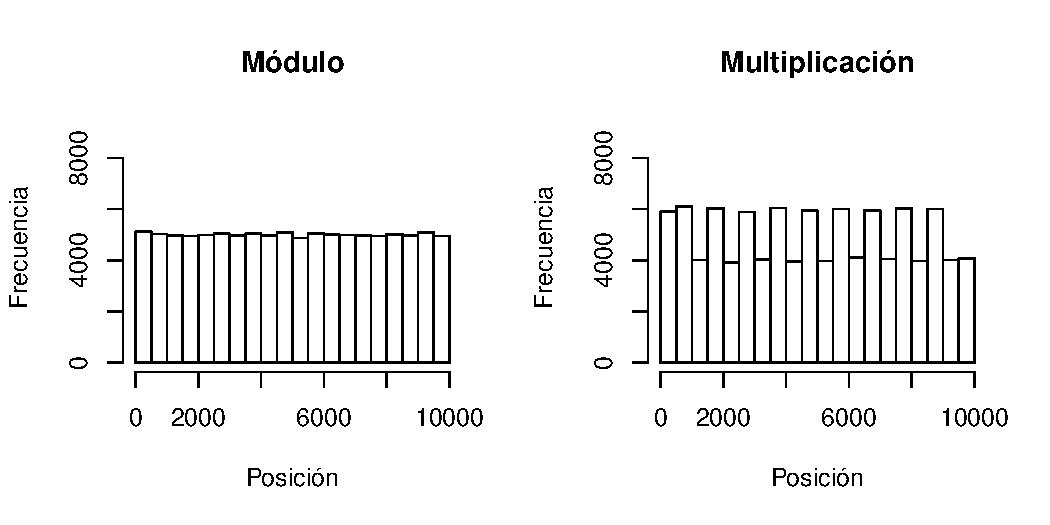
\includegraphics[width=\textwidth]{boxplot_tipo.pdf}
  \caption{Resultado de la experimentación en un proceso de inserción}
  \label{fig:colision}
\end{figure}

Respecto al número de colisiones, el método de división obtiene en promedio entre todas las iteraciones un $56\%$ de colisiones y el método de multiplicación cercano al $88\%$, lo que refuerza el argumento de que la función módulo es eficiente y evita en menor medida el número de colisiones.


\begin{thebibliography}{0} 
\bibitem{Graham1994} R.~L.~Graham, D.~E.~Knuth y O.~Patashnik: \textit{Concrete Mathematics: A Foundation for Computer Science}. Addison Wesley, 1994.
  \bibitem{Knuth1998} Donald Knuth, \textit{Sorting and searching}, The Art of Computer Programming, Addison-Wesley Professional, 1998.
   \bibitem{Papadimitriou1993} Christos H. Papadimitriou, \textit{Computational Complexity}, Addison-Wesley Professional, 1993.
  \bibitem{Schaeffer2020} Elisa Schaeffer, \textit{Modelos computacionales}, Complejidad computacional de problemas y el análisis y diseño de algoritmos, notas de curso, 2020.
\end{thebibliography}



\end{document}


